\chapter{Theoretical background}

This chapter introduces the physical and numerical concepts required to interpret the evolution of the inner dark matter density in ultra-faint dwarf galaxy simulations. The objective is not to review all of modern structure formation, but to establish the framework needed for the analyses in subsequent chapters: collisionless halo dynamics, cusp/core phenomenology, numerical heating, gravitational softening, the gravity solver controls used in SWIFT, and the role of shell-to-shell coupling in mass redistribution.

\section{Dark matter halos and density profiles}
\label{sec:bg_halos_profiles}

In the collisionless limit, dark matter is described by a phase-space distribution function $f(\mathbf{x},\mathbf{v},t)$ that obeys the collisionless Boltzmann equation, coupled to Poisson's equation for the gravitational potential \citep{binney2008galactic}. The key implication is that halo evolution is governed by a smooth mean gravitational field rather than by direct microscopic collisions between particles.

Using standard notation, the collisionless system is governed by
\begin{equation}
\frac{\partial f}{\partial t} + \mathbf{v}\cdot\nabla_{\mathbf{x}} f - \nabla_{\mathbf{x}}\Phi\cdot\nabla_{\mathbf{v}} f = 0,
\end{equation}
with the potential determined by
\begin{equation}
\nabla^2 \Phi = 4\pi G\rho, \qquad \rho(\mathbf{x},t) = \int f(\mathbf{x},\mathbf{v},t)\,\mathrm{d}^3\mathbf{v}.
\end{equation}
These equations make clear that halo structure is a phase-space problem: the density profile cannot be understood independently of the velocity distribution and orbital content.

In cosmological simulations, dynamically relaxed halos are commonly described by broken power-law density profiles, where the logarithmic slope changes from inner to outer radii. In this language, the central shape of the profile is the critical diagnostic: a steep rise toward small radii is referred to as a \emph{cusp}, while a flattened inner profile is referred to as a \emph{core}. Since this inner region is also the most demanding numerically, any physical interpretation must be tied to explicit convergence and resolution arguments \citep{power2003inner,zhang2019optimal}.

A widely used fitting form for collisionless dark matter haloes is the Navarro--Frenk--White (NFW) profile,
\begin{equation}
\rho(r) =
\frac{\rho_s}
{\left(r/r_s\right)\left(1+r/r_s\right)^2},
\end{equation}
where $\rho_s$ is a characteristic density and $r_s$ is the scale radius at which the logarithmic slope changes from approximately $-1$ to $-3$.

A commonly used reference model is the NFW-like form, which captures the transition from an inner and outer power-law regime. The associated local slope,
\begin{equation}
\gamma(r) \equiv -\frac{\mathrm{d}\ln\rho}{\mathrm{d}\ln r},
\end{equation}
is a useful quantity because it directly tracks whether the central profile evolves toward cusp-like or core-like behaviour.

\begin{figure}[H]
	\centering
	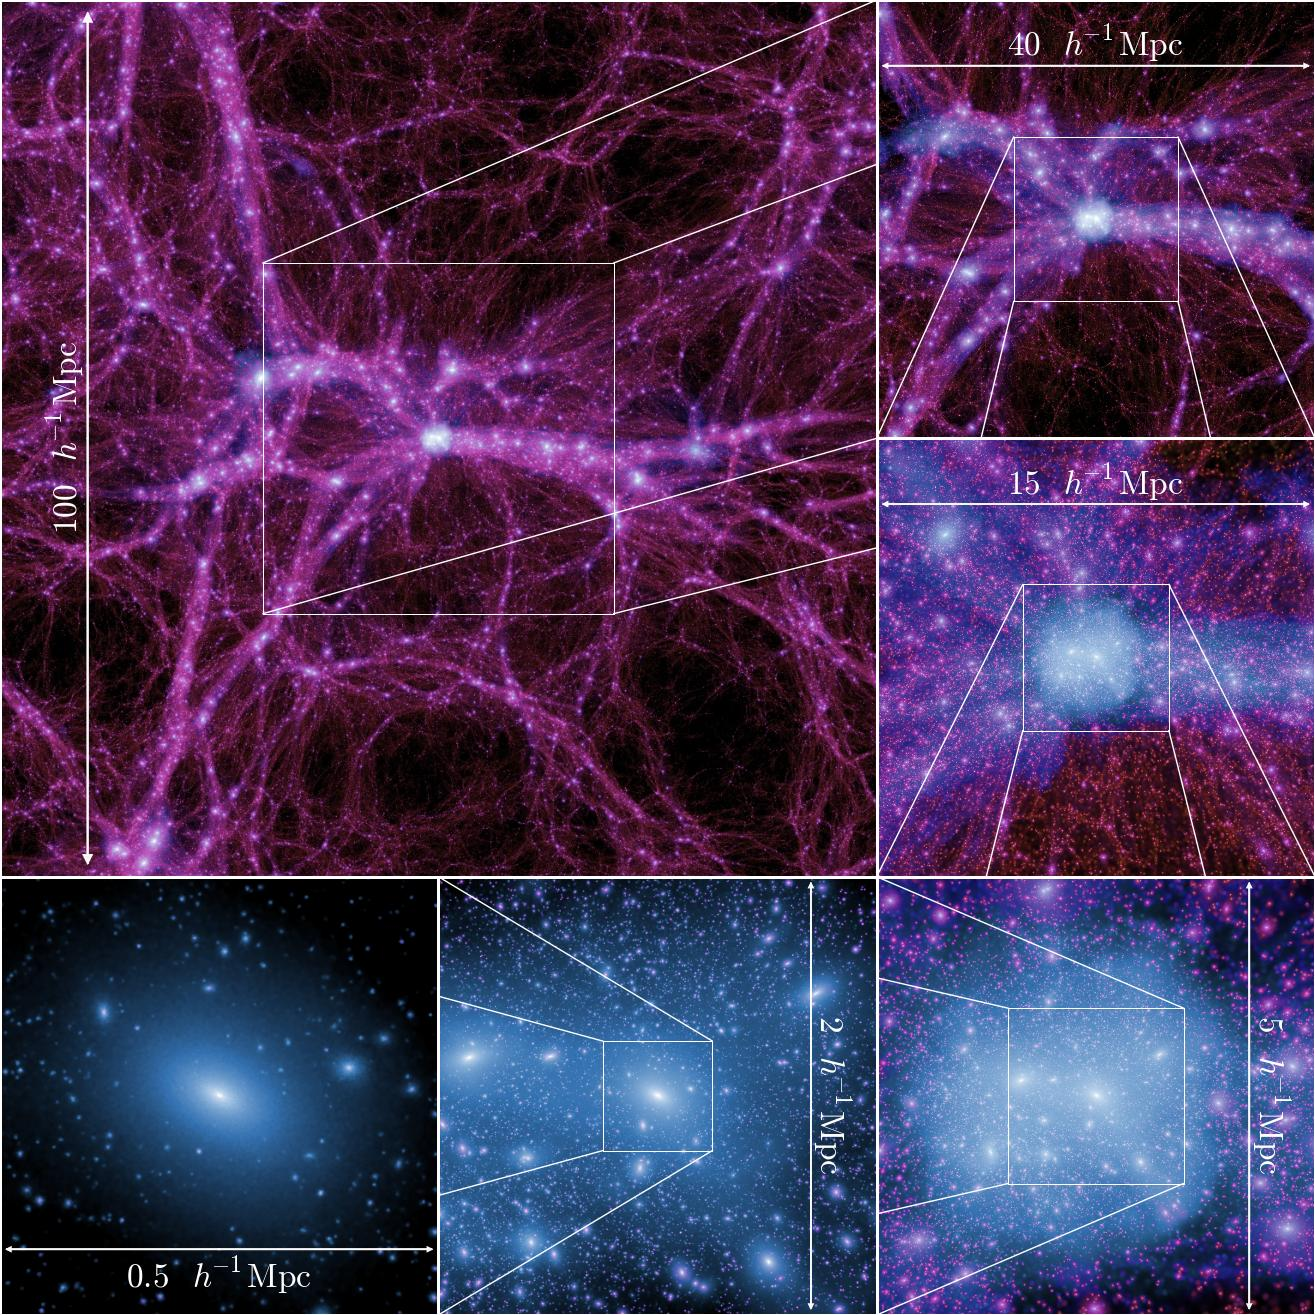
\includegraphics[width=0.8  \textwidth]{content/ch3/img/millennium2zoom_paper.jpg}
	\caption{Zoom sequence (100 to 0.5 Mpc/h) into the most massive halo at $z=0$ from the Millennium-II Simulation \citep{boylan2009millennium2}.}
	\label{fig:millennium2_zoom}
\end{figure}

\subsection{Virial equilibrium, characteristic timescales, and orbital support}
\label{sec:bg_virial_jeans}

Dark matter haloes are not static objects, but many relaxed systems are close enough to dynamical equilibrium that a virial description is useful. 

For a virialized self-gravitating system, the time-averaged kinetic and potential energies approximately satisfy
\begin{equation}
2K + U \approx 0,
\end{equation}
which provides a useful global characterization of dynamical equilibrium.

In that regime, the balance between kinetic and potential energy sets the overall structure of the halo, while the local orbital distribution determines how the inner profile evolves over time. The relevant timescale is the dynamical time,
\begin{equation}
t_{\mathrm{dyn}}(r) \sim \left[G\bar{\rho}(<r)\right]^{-1/2},
\end{equation}
which becomes short in the dense central regions and therefore makes the inner halo especially sensitive to both physical perturbations and numerical error.

A useful way to connect density structure to orbital support is through the spherical Jeans equation,
\begin{equation}
\frac{\mathrm{d}\left(\rho \sigma_r^2\right)}{\mathrm{d}r}
+2\beta(r)\frac{\rho \sigma_r^2}{r}
=
-\rho \frac{\mathrm{d}\Phi}{\mathrm{d}r},
\end{equation}
where $\sigma_r$ is the radial velocity dispersion and $\beta(r)$ is the anisotropy parameter. This equation shows that the density profile cannot be interpreted independently of the velocity structure: two haloes with similar density profiles may differ substantially in orbital content and stability.

Radial anisotropy is particularly important because systems dominated by radial orbits can respond differently to perturbations and secular evolution than more isotropic systems. Changes in orbital anisotropy may therefore accompany or even drive changes in the inner density structure.

\section{Cusp-core behaviour in ultra-faint dwarf galaxies}
\label{sec:bg_cusp_core}

Ultra-faint dwarf galaxies are particularly valuable for small-scale dark matter studies because they are strongly dark-matter dominated and have shallow gravitational potentials. Their internal structure is therefore sensitive both to the underlying dark matter model and to dynamical heating processes that can redistribute mass over time \citep{salamin2026origin}.

In a cold dark matter scenario, cuspy inner profiles are the usual expectation for collisionless halos. In warmer dark matter scenarios, free-streaming suppresses small-scale power and can alter assembly histories, potentially affecting central structure indirectly through different accretion and merger pathways \citep{salamin2026origin}. Independently of the particle model, repeated perturbations and non-adiabatic potential fluctuations can transfer energy to central orbits and drive profile flattening.

The conceptual point is that core formation does not originate from one mechanism. Similar-looking inner profiles can emerge from different routes: altered initial fluctuation spectra, stochastic heating by external perturbers, or numerical relaxation. As a result, interpretation requires combining profile evolution with complementary diagnostics.

This creates a central interpretive challenge for the present work: an apparent cusp-to-core transition can arise from physical mechanisms, from numerical artifacts, or from both acting simultaneously.

\section{Numerical heating and relaxation effects in \texorpdfstring{$N$-body}{N-body} systems}
\label{sec:bg_relaxation}

An $N$-body simulation represents a continuous collisionless fluid with a finite number of massive macro-particles. This discretization introduces spurious collisionality: close encounters can produce artificial two-body relaxation, velocity diffusion, and long-term heating, especially in poorly resolved central regions \citep{binney2008galactic,power2003inner}.

To first order, the local relaxation timescale scales approximately as
\begin{equation}
t_{\mathrm{relax}} \sim \frac{N}{8\ln N}\,t_{\mathrm{cross}},
\end{equation}
where $N$ is the number of effective particles supporting the region of interest and $t_{\mathrm{cross}}$ is a characteristic crossing time \citep{binney2008galactic}. This scaling emphasizes why central halo regions are vulnerable: they contain fewer particles and shorter dynamical times, making discreteness effects comparatively stronger.

The classical relaxation timescale argument provides a first-order test: if the numerical relaxation time at a given radius is not much longer than the simulated evolution time, then the resulting structure may be numerically biased.

Power et al. translated these ideas into practical convergence guidance for halo simulations by linking reliability in the inner profile to a combination of mass resolution, timestep sampling, and force softening \citep{power2003inner}. Their framework remains a benchmark because it moves beyond single-parameter tuning and treats convergence as a coupled numerical problem.

For this thesis, numerical heating is not treated as a generic warning but as an explicit hypothesis to test. If central density decline is dominated by relaxation artifacts, it should correlate with changes in numerical controls. If it persists across broad parameter changes, a more global dynamical mechanism becomes more plausible.

\section{Gravitational softening: fixed and adaptive formulations}
\label{sec:bg_softening}

Gravitational softening modifies the short-range Newtonian force to prevent unphysical singular accelerations from particle-particle encounters. With a fixed softening length $\epsilon$, one obtains a trade-off: large $\epsilon$ suppresses noise and relaxation but erases genuine small-scale structure; small $\epsilon$ improves nominal resolution but can increase heating \citep{power2003inner,zhang2019optimal}.

In many implementations, this can be written schematically with a softened pair force,
\begin{equation}
\mathbf{F}_{12} = -\frac{Gm_1m_2}{\left(r_{12}^2+\epsilon^2\right)^{3/2}}\,\mathbf{r}_{12},
\end{equation}
which regularizes the $r^{-2}$ singularity at very short separation \citep{zhang2019optimal}. The interpretation of $\epsilon$ is therefore two-fold: it is both a numerical stabilizer and a scale that limits physically meaningful force gradients.

Power et al. established influential convergence criteria linking softening, timestep, and particle number in the inner halo \citep{power2003inner}. Later work showed that these prescriptions may be conservative for some setups, while also emphasizing that excessively small softening can bias the innermost density high \citep{zhang2019optimal}. Taken together, these studies show that softening is not a single "best" number independent of context.

Adaptive softening addresses this by varying effective force resolution with local conditions. However, straightforward implementations do not preserve conservation laws. The Lagrangian formalism of Price and Monaghan demonstrated how to construct adaptive softening with the additional correction terms required for consistent energy and momentum conservation \citep{price2007energy}. Modern conservative extensions generalize this framework to multi-species collisionless simulations \citep{hopkins2023novel}.

From a methodological perspective, adaptive schemes are especially relevant for halos with strong radial density contrasts. A fixed $\epsilon$ that is adequate in the outskirts may be too coarse in the center, while an $\epsilon$ tuned to the center may be too noisy at large radii. Conservative adaptive formulations provide a way to mitigate this tension while preserving the invariants required for long integrations.

In the context of this thesis, softening is a key control variable which will be studied in detail.

\section{Gravity solver controls in SWIFT}
\label{sec:bg_solver_controls}

Beyond softening, force computation in modern cosmological codes depends on hierarchical gravity solvers (tree and fast multipole expansions) and their acceptance criteria. These methods accelerate long-range gravity by replacing exact pairwise summation with controlled approximations, whose errors depend on opening criteria and expansion tolerances.

This introduces a second numerical layer on top of softening. Even with identical initial conditions and identical softening, changes in opening criteria or multipole tolerances can alter force errors in a way that accumulates over many dynamical times. For slowly evolving central densities, small systematic differences can integrate into measurable secular trends.

In practical terms, parameters such as the multipole acceptance criterion (MAC), geometric opening thresholds (e.g. $\theta_{\mathrm{cr}}$), expansion tolerances (e.g. FMM error controls), and timestep factors set the balance between computational cost and force accuracy. Because central density evolution is sensitive to small cumulative force biases, these controls must be included in any sensitivity analysis of cusp/core evolution.

The same logic applies to timestep controls. If timesteps are too large compared to local orbital times, integration error can mimic diffusion or heating. If they are too small, the simulation becomes expensive but not necessarily more accurate unless force errors are also reduced. A reliable interpretation therefore requires tests across both integration and force-approximation parameters.

\begin{figure}[H]
	\centering
	\begin{minipage}[t]{0.48\textwidth}
		\centering
		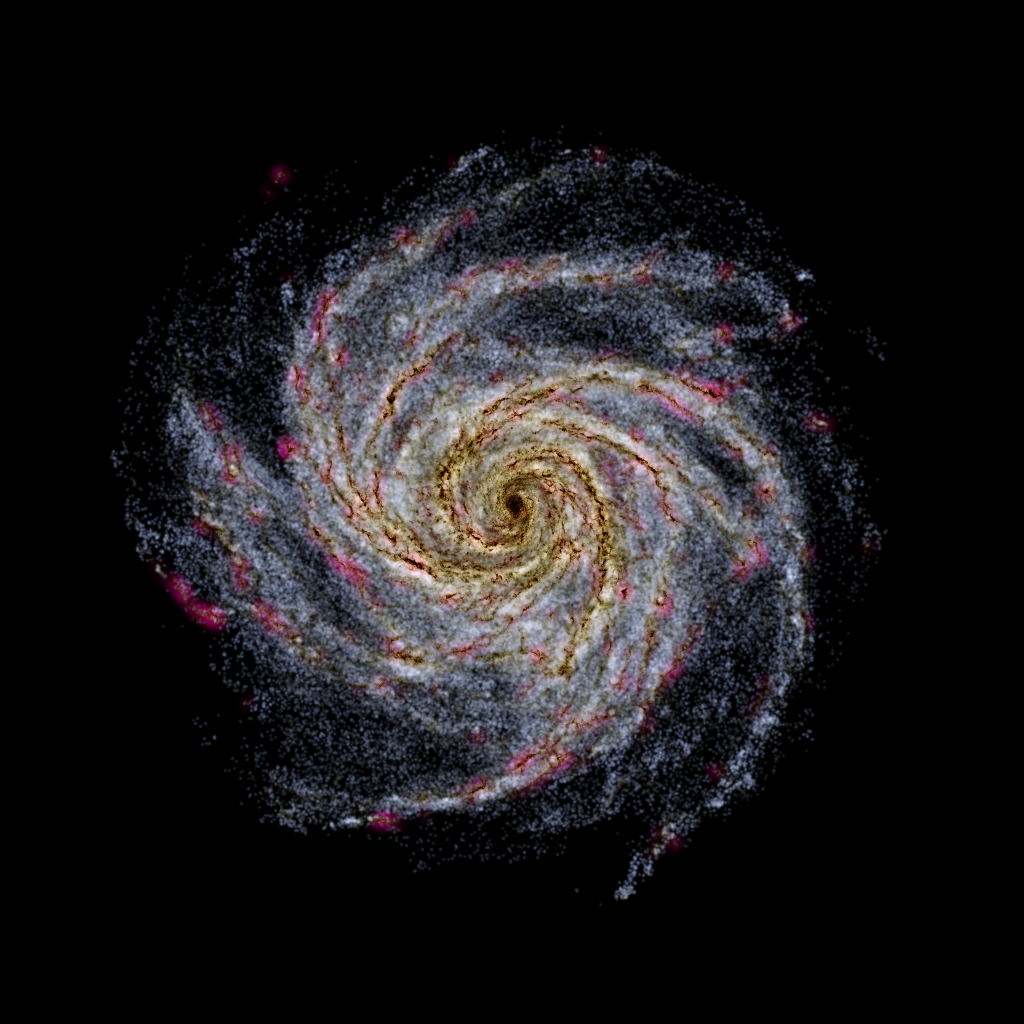
\includegraphics[width=\linewidth]{content/ch3/img/agora_gear_revaz.png}
		{\small\textit{Agora galaxy (GEAR model). A simulation highlighting gas, star formation and morphological features produced with the GEAR physics module. Image: Yves Revaz, SWIFT gallery.}}
	\end{minipage}\hfill
	\begin{minipage}[t]{0.48\textwidth}
		\centering
		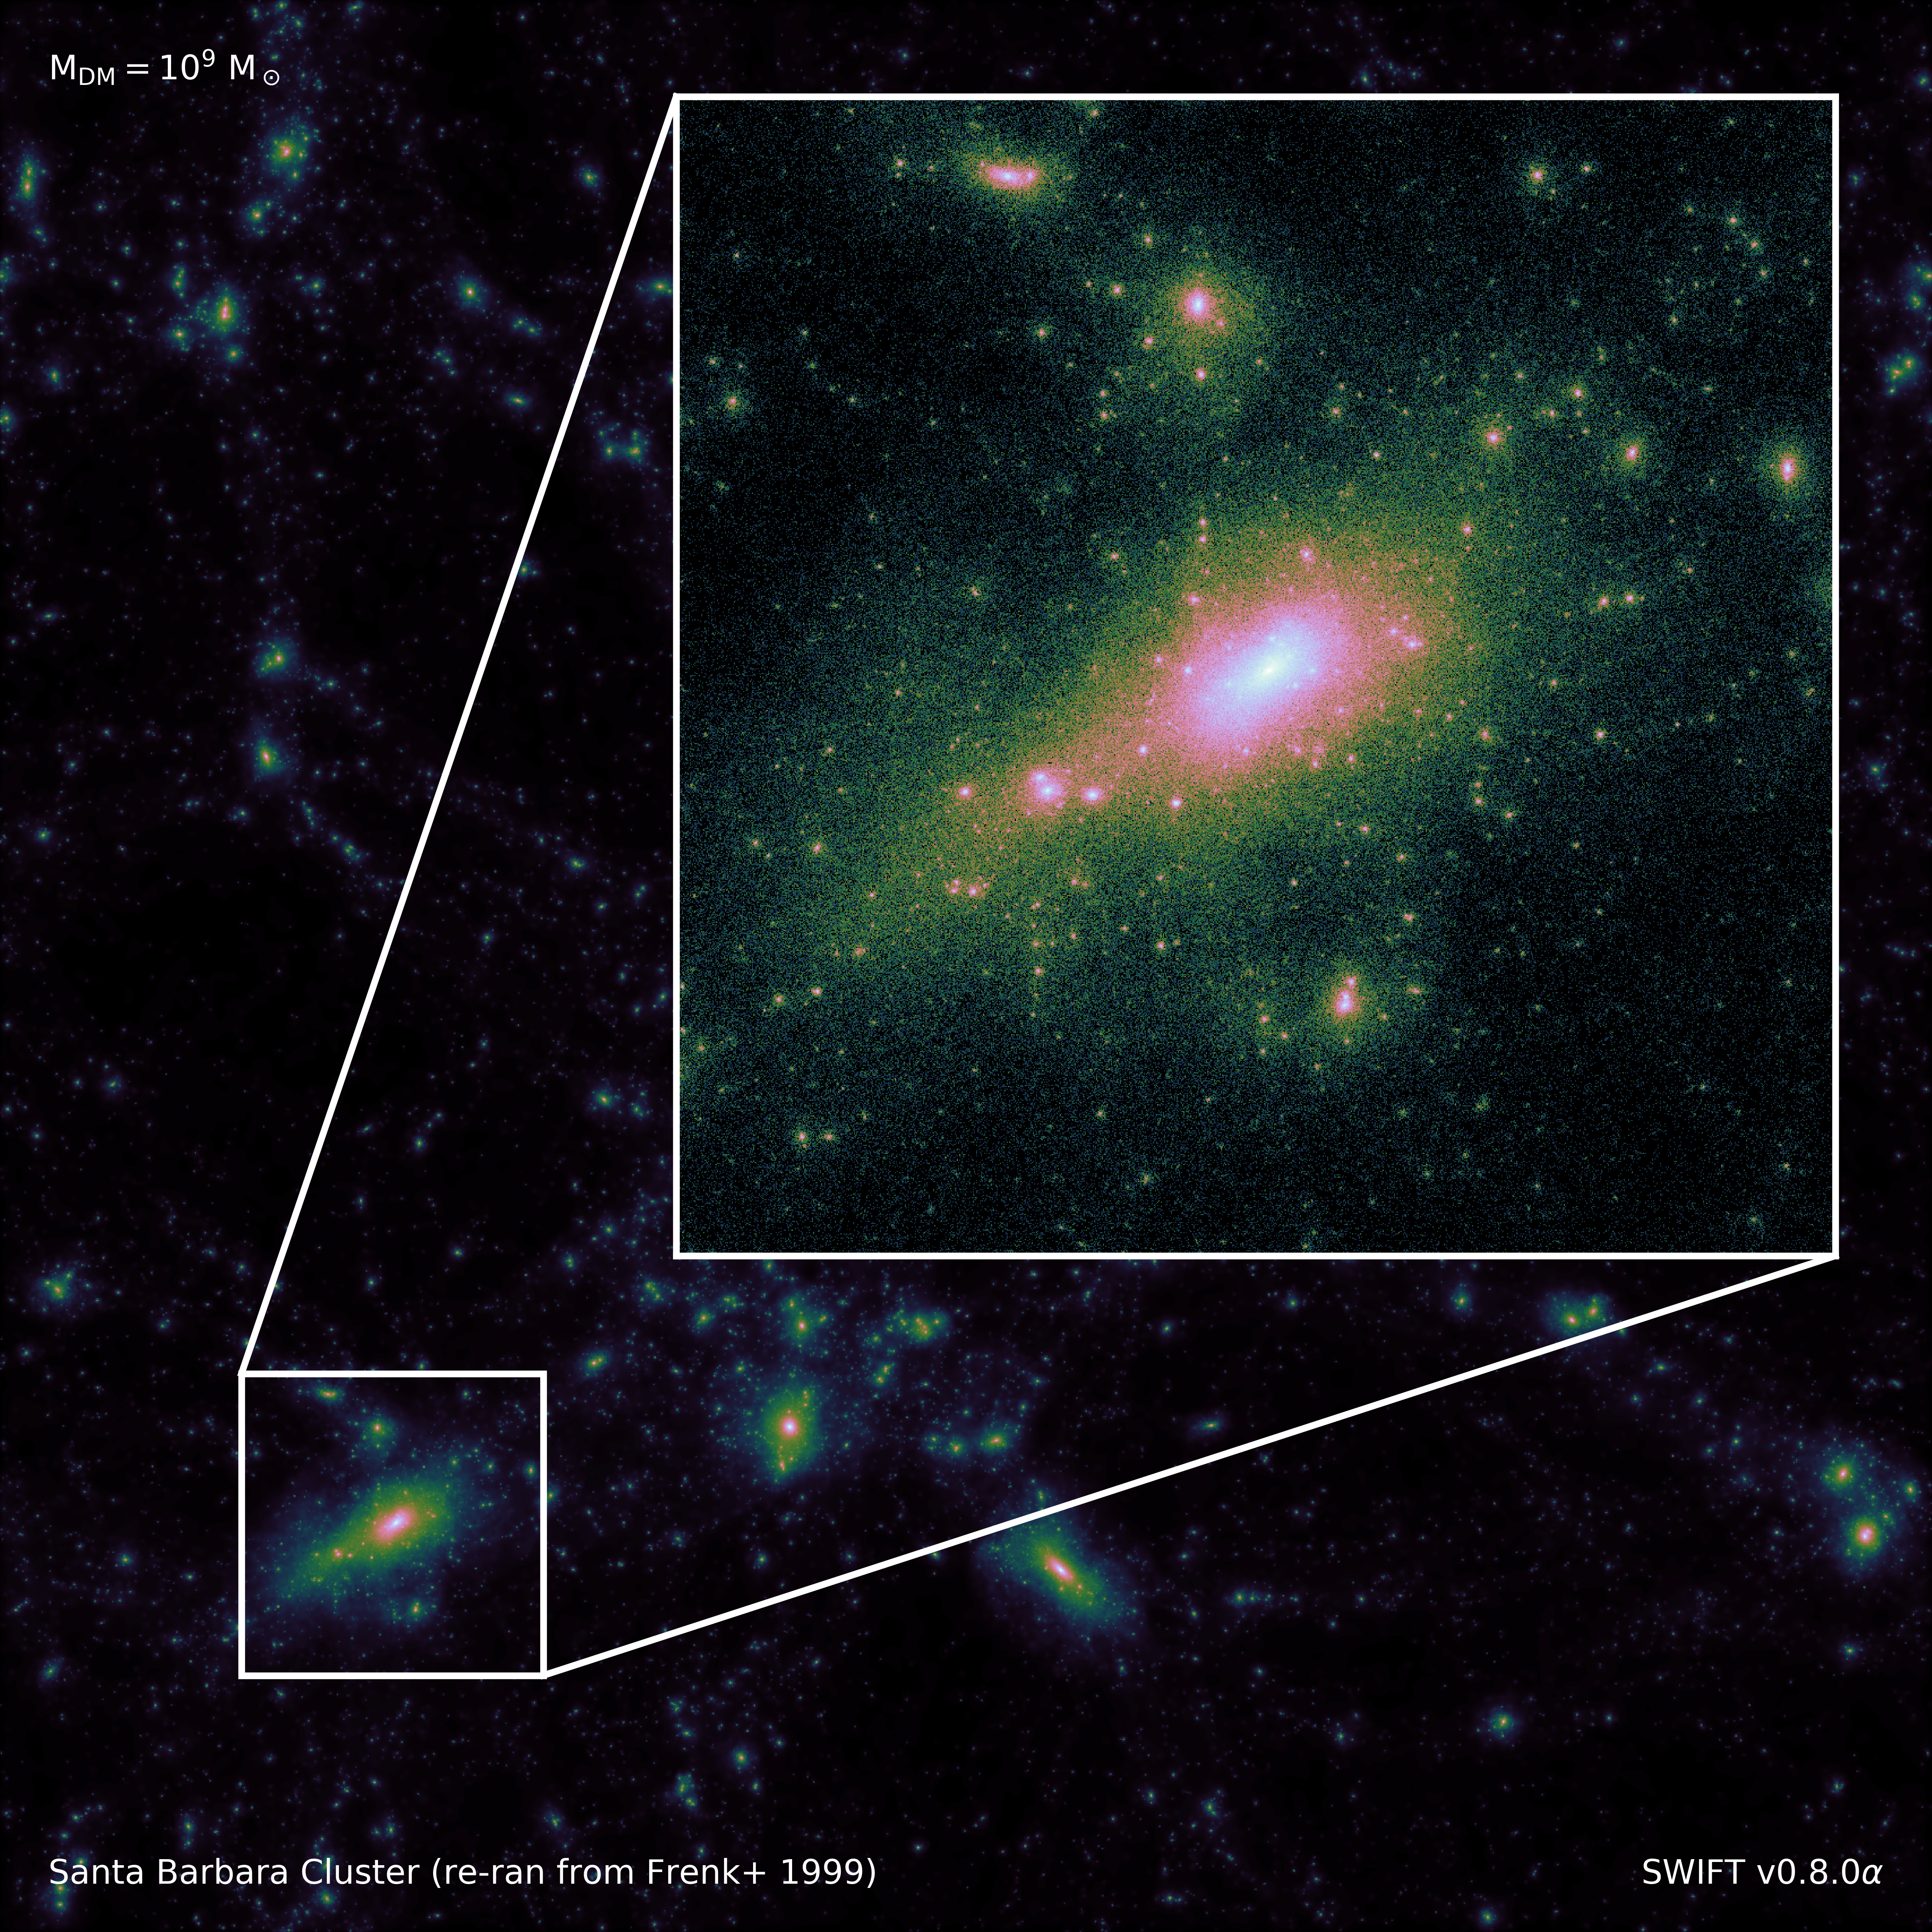
\includegraphics[width=\linewidth]{content/ch3/img/santa_barbara_borrow.png}
		{\small\textit{Santa-Barbara Cluster. A large-scale cluster formation snapshot from the Santa Barbara comparison suite. Image: Josh Borrow, SWIFT gallery.}}
	\end{minipage}
	\caption{Simulation examples from the SWIFT gallery \citep{swiftgallery2024}.}
	\label{fig:swift_gallery_examples}
\end{figure}

\section{Why shell structure and mass redistribution matter}
\label{sec:bg_shells}

A central point for this thesis is that inner density evolution is not purely local. Even when interest focuses on the innermost region, the central potential is influenced by mass and orbital structure over a broad radial range. Particle populations at larger radii can contribute to central acceleration fluctuations, angular momentum exchange, and gradual redistribution of enclosed mass.

Recent theoretical work on stochastic tidal fields generated by clumpy substructure provides a useful interpretation for this non-local coupling. In these treatments, gravitational fluctuations induce diffusion in orbital integrals and can transfer energy and angular momentum through repeated perturbations rather than through single events \citep{penarrubia2019stochastic,penarrubia2017fluctuations}.

An important implication is that central density decline may be driven by the full halo environment, not only by the innermost force law. If true, changing local softening alone may leave a substantial part of the trend unchanged. This is precisely why shell-resolved measurements and cumulative mass diagnostics are central to the thesis design.

This motivates a shell-based analysis in which the halo is decomposed into radial regions and their dynamical influence on the center is tracked over time. If outer shells contribute substantially to central kinematic evolution, then changing only inner local parameters (for example, local softening) may have limited impact on the global trend.

This non-local perspective is consistent with previous findings in the project context, where persistent central density decline can remain visible across multiple numerical variations \citep{salamin2026origin}.

\subsection{Global coupling through the halo potential}
\label{sec:bg_global_coupling}

Although the radial force inside a spherical shell depends only on the mass enclosed within that radius, the potential and orbital structure of the system still reflect the full mass distribution. For a spherically symmetric halo,
\begin{equation}
g(r) = -\frac{G M(<r)}{r^2},
\end{equation}
while the potential can be written schematically as
\begin{equation}
\Phi(r) = -G\left[\frac{M(<r)}{r} + \int_r^\infty \frac{1}{r'}\,\mathrm{d}M(r')\right].
\end{equation}
This distinction is important: outer shells do not change the local radial force inside them, but they do contribute to the depth of the potential well and to the overall orbital environment of inner particles.

The consequence is that central evolution cannot be assumed to be purely local. Even if the inner density is the observable of interest, outer regions may still influence it through the global potential, through cumulative mass redistribution, and through long-term coupling of orbital structure. This is the theoretical basis for the shell-resolved diagnostics used later in the thesis.
